\documentclass[12pt]{article}
\usepackage[a4paper,margin=1in,showframe]{geometry}
\usepackage{tikz}
\usetikzlibrary{
  chains,
  shapes.multipart,
}
\begin{document}
\begin{figure}[!ht]
\centering
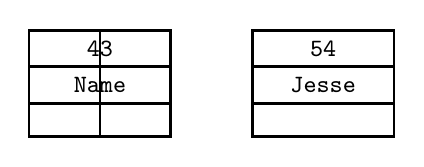
\begin{tikzpicture}[
  line width=1pt,
  font=\small\ttfamily,
  list/.style={
     rectangle split,
     rectangle split parts=3,
     draw,
     minimum width=1.8cm,
  },
  start chain,
  chain default direction=down
]
   \node[list,on chain] (A) {43 \nodepart{two} Name}; 
   \draw (A.three north) -- (A.three south);
   \node[list,on chain] (B) {54 \nodepart{two} Jesse}; 
\end{tikzpicture}
\end{figure}
\end{document} 